\documentclass[a4paper,dvipdfmx,10.5pt]{jarticle}
%使うパッケージ
\usepackage{physics,amsmath,amssymb,amsfonts,mathtools,ulem}
\usepackage{siunitx}
\usepackage[thicklines]{cancel}
\usepackage[dvipdfmx]{graphicx}
\usepackage[dvipdfmx]{color}
%\graphicspath{{./result/},{./picture/}}
\usepackage{layout}
\usepackage{here}
\usepackage{bm}
\usepackage{url}
\usepackage{ascmac}
\usepackage{tikz}
\usepackage{amsthm}
\usetikzlibrary{intersections,calc,arrows.meta}
\usepackage[hang,small,bf]{caption}
\usepackage[subrefformat=parens]{subcaption}
\captionsetup{compatibility=false}
\usepackage[margin=20truemm]{geometry}
\usepackage[dvipdfmx]{hyperref}
\usepackage{pxjahyper} % (u)pLaTeXのときのみかく
\hypersetup{%
 setpagesize=false,%
 bookmarks=true,%
 bookmarksdepth=tocdepth,%
 bookmarksnumbered=true,%
 colorlinks=true,%
 linkcolor=blue
}
% タイトル,著署名,日付
\title{大学院 物理基本実験\\テーマA: 原子の分光と量子力学}
\author{関澤研究室\\26M00623\\田中 大智}
\date{\today}
% 体裁の設定
\setlength{\oddsidemargin}{0pt}
\setlength{\textwidth}{453pt}
\setlength{\marginparwidth}{18pt}
\setlength{\marginparsep}{18pt}



%%%%%%%%%%%%%%%%%%%%%%%%本文%%%%%%%%%%%%%%%%%%%%%%%%%%%%%
\begin{document}

\maketitle
\section{目的}
 原子は原子核と電子から構成され，原子核は陽子と中性子から構成されている．電子は原子核の周りに存在する特定のエネルギー準位に対応する電子軌道に束縛されている．電子のエネルギー準位は量子力学的な性質を持ち，特定のエネルギー差を持つ電子遷移が起こると，特定の波長の光が放出される．このエネルギー準位の差の計算は水素原子についてはシュレーディンガー方程式を解くことで行われるが，ヘリウム原子のような多電子原子では電子間の相互作用が複雑であるため，摂動法や変分法などの近似的な方法が必要となる．

 本実験では，以下の2点を目的として実験を行った．まず第一に水素原子のスペクトルはシュレーディンガー方程式を解き，ヘリウム原子については近似法を用いてスペクトルを計算し，これとスペクトル線の測定結果を比較した．第二に加えてLED，白熱電球，水銀灯のスペクトルといった様々な光源のスペクトルを観測することであった．
\section{原理}
\subsection{水素原子のスペクトル}
水素原子は1個の電子と1個の陽子から構成されている．水素原子のスペクトルは，可視光領域がバルマーによって，紫外線領域がライマンによって，赤外線領域がパッシェンによって発見された．これらのスペクトル線は，電子が特定のエネルギー準位から別のエネルギー準位に遷移する際に放出される光の波長を表している．水素原子のスペクトル線の波長は，リュードベリ定数を用いて以下の式で表される．
\begin{equation}
  \frac{1}{\lambda} = R_H \left( \frac{1}{n_1^2} - \frac{1}{n_2^2} \right).\label{eq:Rydberg}
\end{equation}
ここで，$\lambda$はスペクトル線の波長，$R_H=1.097 \times 10^7 \, \text{m}^{-1}$は水素原子のリュードベリ定数，$n_1$と$n_2$は電子のエネルギー準位を表す整数である．

式\eqref{eq:Rydberg}はシュレーディンガー方程式を解くことで導かれる．シュレーディンガー方程式は，量子力学において粒子の波動関数を記述する基本的な方程式である．水素原子の場合，相対運動のシュレーディンガー方程式は以下のように表される．
\begin{equation}
  \left[-\frac{\hbar^2}{2m} \laplacian  - \frac{e^2}{4\pi \epsilon_0 r} \right] \psi(\mathbf{r}) = E \psi(\mathbf{r}).\label{eq:Schrodinger}
\end{equation}
ここで，$\hbar$はディラック定数，$m$は電子の換算質量，$\epsilon_0$は真空の誘電率，$r$は電子と原子核との距離である．$\psi(\mathbf{r})=u_{nl}(r) Y_{lm}(\theta, \phi)/r$と分離して得られる動径方向のシュレーディンガー方程式とそれに冪級数を代入し，無限遠での境界条件を適用することでエネルギー準位が求まる．動径方向のシュレーディンガー方程式とエネルギー準位は以下のように表される．
\begin{align}
  &\left[-\frac{\hbar^2}{2m} \dv[2]{r} + \frac{\hbar^2}{2m}\frac{ l(l+1)}{r^2} - \frac{e^2}{4\pi \epsilon_0 r} \right] u_{nl}(r) = E u_{nl}(r).\label{eq:radial}\\
  &E_n = - \frac{mc^2}{2}\alpha^2\frac{1}{n^2}\simeq -13.6\frac{1}{n^2} \, \text{eV}.\label{eq:energy}\\
  &\frac{u_{nl}(r)}{r}= -\frac{2}{n^2}\frac{1}{a_0^{3/2}}\sqrt{\frac{(n-l-1)!}{[(n+l)!]^3}}\rho^l L_{n+l}^{2l+1}\exp(-\frac{1}{2}\rho).\label{eq:radial_solution}
\end{align}
ここで，$l$は軌道角運動量量子数，$n$は主量子数，$\alpha= \frac{e^2}{4\pi \epsilon_0 \hbar c} \approx \frac{1}{137}$は微細構造定数である．式\eqref{eq:energy}から，水素原子のエネルギー準位は主量子数$n$のみに依存し，スペクトル線の波長も式\eqref{eq:Rydberg}のように$n_1$と$n_2$のみに依存することがわかる．特に基底状態の波動関数は$n=1$，$l=0$のときであり，以下のように表される．
\begin{equation}
  \psi_{100}(\mathbf{r}) = \frac{1}{\sqrt{\pi a_0^3}} \exp(-\frac{r}{a_0}).\label{eq:ground_state}
\end{equation}
\subsection{ヘリウム原子のスペクトル}
\subsubsection{相互作用項を無視した場合}
ヘリウム原子のシュレーディンガー方程式は以下のように表される．
\begin{equation}
  \left[-\frac{\hbar^2}{2m} \laplacian_1 - \frac{\hbar^2}{2m} \laplacian_2 - \frac{2e^2}{4\pi \epsilon_0 r_1} - \frac{2e^2}{4\pi \epsilon_0 r_2} + \frac{e^2}{4\pi \epsilon_0 r_{12}} \right] \psi(\mathbf{r}_1, \mathbf{r}_2) = E \psi(\mathbf{r}_1, \mathbf{r}_2)\,.\label{eq:He_Schrodinger}
\end{equation}
ここで，$\laplacian_1$と$\laplacian_2$はそれぞれの電子のラプラシアン演算子，$r_1$と$r_2$はそれぞれの電子と原子核との距離，$r_{12}$は2つの電子間の距離である．相互作用項を無視すると，変数分離ができて$e\to2e$としたときの水素原子の方程式を2つ解くことになる．なお，その方程式は以下のように導出される．
\begin{align}
  H\psi_1(\mathbf{r}_1)\psi_2(\mathbf{r}_2) &= \psi_2(\mathbf{r}_2) \left[-\frac{\hbar^2}{2m} \laplacian_1 - \frac{2e^2}{4\pi \epsilon_0 r_1} \right] \psi_1(\mathbf{r}_1) + \psi_1(\mathbf{r}_1) \left[-\frac{\hbar^2}{2m} \laplacian_2 - \frac{2e^2}{4\pi \epsilon_0 r_2} \right] \psi_2(\mathbf{r}_2)\\
  &=E_1 \psi_1(\mathbf{r}_1)\psi_2(\mathbf{r}_2) + E_2 \psi_1(\mathbf{r}_1)\psi_2(\mathbf{r}_2).
\end{align}
よって，以下の2つのシュレーディンガー方程式を解くことになる．
\begin{align}
  &\left[-\frac{\hbar^2}{2m} \laplacian_1 - \frac{2e^2}{4\pi \epsilon_0 r_1} \right] \psi_1(\mathbf{r}_1) = E_1 \psi_1(\mathbf{r}_1),\\
  &\left[-\frac{\hbar^2}{2m} \laplacian_2 - \frac{2e^2}{4\pi \epsilon_0 r_2} \right] \psi_2(\mathbf{r}_2) = E_2 \psi_2(\mathbf{r}_2).
\end{align}
この場合，エネルギー準位は以下のように表される．
\begin{equation}
  E_{n_1 n_2} \simeq -54.4 \left( \frac{1}{n_1^2} + \frac{1}{n_2^2} \right) \, \text{eV}.\label{eq:He_energy_no_interaction}
\end{equation}
\subsubsection{相互作用項を摂動項とした場合}
式\eqref{eq:He_Schrodinger}の左辺について，第4項までを非摂動項$H_1$，第5項を摂動項$H_2$とする．非摂動項$H_1$の固有関数は，水素様原子の固有関数の積で表される．このとき，非摂動項$H_1$のエネルギー準位$E_1$は式\eqref{eq:He_energy_no_interaction}で表され，その基底状態のエネルギーは$n_1=n_2=1$のときである．また，$H_1$に対する基底状態の波動関数は式\eqref{eq:ground_state}の原子番号を$1\to 2$としたときのものの積で表される．このとき，基底状態の波動関数は以下のように表される．
\begin{equation}
  \psi_{100}(\mathbf{r}_1)\psi_{100}(\mathbf{r}_2) = \frac{8}{\pi a_0^3} \exp\left(-\frac{2(r_1 + r_2)}{a_0}\right)\,.\label{eq:He_ground_state_no_interaction} 
\end{equation}
一次の摂動エネルギーは，式\eqref{eq:He_ground_state_no_interaction}について摂動項$H_2$の期待値を取ることで求まる．このとき，式\eqref{eq:He_perturbation_energy}のように表される．
\begin{align}
  E_2&= \bra{\psi_{100}(\mathbf{r}_1)\psi_{100}(\mathbf{r}_2)} H_2 \ket{\psi_{100}(\mathbf{r}_1)\psi_{100}(\mathbf{r}_2)}\label{eq:He_perturbation_energy_1}\\
  &= \int \dd[3]{r_1} \int \dd[3]{r_2} \frac{8}{\pi a_0^3} \exp\left(-\frac{2(r_1 + r_2)}{a_0}\right) \frac{e^2}{4\pi \epsilon_0 r_{12}} \frac{8}{\pi a_0^3} \exp\left(-\frac{2(r_1 + r_2)}{a_0}\right)\\ 
  & = \frac{e^2}{4\pi \epsilon_0} \left( \frac{8}{\pi a_0^3}\right)^2 \int \dd[3]{r_1} \exp\left(-\frac{4r_1}{a_0}\right) \uwave{\int \dd[3]{r_2} \exp\left(-\frac{4r_2}{a_0}\right) \frac{1}{r_{12}}}\,.\label{eq:He_1st_order1}
\end{align}
まず，式\eqref{eq:He_1st_order1}の波線部について考える．この部分について，球面座標系を導入し，$\theta$を$r_2$と$r_1$のなす角とすると，以下のように表される．
\begin{align}
  &\quad \int \dd[3]{r_2} \exp\left(-\frac{4r_2}{a_0}\right) \frac{1}{r_{12}}\\
  &= \int_0^\infty \dd{r_2} r_2^2 \exp\left(-\frac{4r_2}{a_0}\right) \int_0^\pi \dd{\theta} \sin\theta \int_0^{2\pi} \dd{\phi} \frac{1}{\sqrt{r_1^2 + r_2^2 - 2r_1 r_2 \cos\theta}}\\
  &= 2\pi \int_0^\infty \dd{r_2} r_2^2 \exp\left(-\frac{4r_2}{a_0}\right) \frac{1}{r_1 r_2} \left(r_1+r_2 - \abs{r_1-r_2}\right)\\
  &= \frac{4\pi}{r_1} \int_0^{r_1} \dd{r_2} r_2^2 \exp\left(-\frac{4r_2}{a_0}\right) + 4\pi \int_{r_1}^\infty \dd{r_2} r_2 \exp\left(-\frac{4r_2}{a_0}\right)\\
  &= \frac{a_0^3\pi}{8r_1}\left[1-\left(1+\frac{2r_1}{a_0}\right)\exp(-\frac{4r_1}{a_0})\right] \,.
  \label{eq:He_1st_order2}
\end{align}
式\eqref{eq:He_1st_order2}を式\eqref{eq:He_1st_order1}に代入し，さらに$r_1$についての積分を行うと，以下のように表される．
\begin{align}
  E_2 &= \frac{e^2}{4\pi \epsilon_0} \left( \frac{8}{\pi a_0^3}\right)^2 \frac{a_0^3\pi}{8} \int_0^\infty \dd{r_1} r_1 \exp\left(-\frac{4r_1}{a_0}\right) \left[1-\left(1+\frac{2r_1}{a_0}\right)\exp(-\frac{4r_1}{a_0})\right]\int_0^{\pi}\sin\theta\dd{\theta}\int_{0}^{2\pi} \dd{\phi} \\
  &= \frac{5}{4} \frac{e^2}{4\pi \epsilon_0 a_0} \,.\label{eq:He_perturbation_energy}
\end{align}
式\eqref{eq:He_energy_no_interaction}と式\eqref{eq:He_perturbation_energy}を用いて，相互作用項を摂動項とした場合のヘリウム原子のエネルギー準位は以下のように表される．
\begin{equation}
  E_{n_1 n_2} \simeq -54.4 \left( \frac{1}{n_1^2} + \frac{1}{n_2^2} \right) + \frac{5}{4} \frac{e^2}{4\pi \epsilon_0 a_0} \, \text{eV}.\label{eq:He_energy_first_order}
\end{equation}
ここに$n_1=n_2=1$のときのエネルギー準位は約-74.83eVとなる．
\subsubsection{変分法を用いた場合}
変分法を用いてヘリウム原子のエネルギー準位を求めることもできる．この場合，試行関数を以下のように式\eqref{eq:He_ground_state_no_interaction}について原子番号を$2\to Z$としたときのものを考えればよく，
\begin{equation}
  \psi(\mathbf{r}_1, \mathbf{r}_2) = \frac{Z^3}{\pi a_0^3} \exp\left(-\frac{Z(r_1 + r_2)}{a_0}\right)\,.\label{eq:He_trial_wavefunction}
\end{equation}
ここで，$Z$は変分パラメータである．この試行関数について，ヘリウム原子のハミルトニアンの期待値を取ることでエネルギー準位を求めることができる．このとき，試行関数は規格化されているので分母を無視できてエネルギー準位は以下のように表される．
\begin{align}
  E(Z) &= \bra{\psi} H \ket{\psi} \\
       &=  \int \dd[3]{r_1} \int \dd[3]{r_2} \psi(\mathbf{r}_1, \mathbf{r}_2)\left[-\frac{\hbar^2}{2m} \laplacian_1  - \frac{2e^2}{4\pi \epsilon_0 r_1} - \frac{\hbar^2}{2m} \laplacian_2- \frac{2e^2}{4\pi \epsilon_0 r_2} + \frac{e^2}{4\pi \epsilon_0 r_{12}} \right] \psi(\mathbf{r}_1, \mathbf{r}_2)\\
       &= \int \dd[3]{r_1} \int \dd[3]{r_2} \psi(\mathbf{r}_1, \mathbf{r}_2) \left[h_1 + h_2 + \frac{e^2}{4\pi \epsilon_0 r_{12}} \right] \psi(\mathbf{r}_1, \mathbf{r}_2)
        \,.\label{eq:He_variational_1}
\end{align}
ここで，
\begin{equation}
  h_i = -\frac{\hbar^2}{2m} \laplacian_i - \frac{2e^2}{4\pi \epsilon_0 r_i}
\end{equation}
である．式\eqref{eq:He_variational_1}の各項について積分を行う．まず，式\eqref{eq:He_variational_1}の最初の2項については添え字の入れ替えに対して対称であることから，積分結果は同じになる．このため，式\eqref{eq:He_variational_1}の1項目について積分を行うだけでよく，
\begin{align}
  \left(\text{1項目}\right) &= \left(\frac{Z^3}{\pi a_0^3}\right)^2 \int \dd[3]{r_1} \int \dd[3]{r_2} \exp\left(-\frac{Z(r_1 + r_2)}{a_0}\right) h_1 \exp\left(-\frac{Z(r_1 + r_2)}{a_0}\right)\label{eq1}\\
  &= \left(\frac{Z^3}{\pi a_0^3}4\pi\right)^2 \int_0^\infty \dd{r_1} r_1^2 \int_0^\infty \dd{r_2} r_2^2 \exp\left(-\frac{Z(r_1 + r_2)}{a_0}\right) \frac{-\hbar^2}{2m} \frac{1}{r_1^2} \dv{}{r_1}\left(r_1^2 \dv{}{r_1}\right) \exp\left(-\frac{Z(r_1 + r_2)}{a_0}\right)\notag\\
  &\quad + \left(\frac{Z^3}{\pi a_0^3}4\pi\right)^2 \int_0^\infty \dd{r_1} r_1^2 \int_0^\infty \dd{r_2} r_2^2 \exp\left(-\frac{Z(r_1 + r_2)}{a_0}\right) \left(-\frac{2e^2}{4\pi \epsilon_0 r_1}\right) \exp\left(-\frac{Z(r_1 + r_2)}{a_0}\right)\label{eq2}\\
  &= -\frac{8\pi e^2}{\epsilon_0}\int_{0}^\infty \dd{r_1}  \int_0^\infty \dd{r_2} r_1r_2^2 \exp\left(-\frac{Z(r_1 + r_2)}{a_0}\right)\notag\\
  &\quad -\frac{8\hbar^2\pi^2}{m}\int_0^\infty \dd{r_1} \int_0^\infty \dd{r_2} 2r_1r_2^2\left(-\frac{Z}{a_0}\right) \exp\left(-\frac{Z(r_1 + r_2)}{a_0}\right)\notag\\
  &\quad -\frac{8\hbar^2\pi^2}{m}\int_0^\infty \dd{r_1} \int_0^\infty \dd{r_2} r_1^2 r_2^2 \left(\frac{Z^2}{a_0^2}\right) \exp\left(-\frac{Z(r_1 + r_2)}{a_0}\right)\\
  &= -\frac{Ze^2}{2\pi\epsilon_0 a_0} + \frac{Z^2\hbar^2}{2m a_0^2}\\
  &= \frac{e^2}{4\pi \epsilon_0 a_0} \left(-2Z + \frac{1}{2}Z^2\right)\,.\label{eq:He_variational_2}
\end{align}
式\eqref{eq1}から式\eqref{eq2}への変形では，球面座標系を導入している．
第3項目については式\eqref{eq:He_perturbation_energy_1}について$2\to Z$としたときの積分結果を用いることで以下のように表される．
\begin{equation}
  \left(\text{3項目}\right) = \frac{5}{8} \frac{Z e^2}{4\pi \epsilon_0 a_0}\,.\label{eq:He_variational_3}
\end{equation}
式\eqref{eq:He_variational_2}を2倍し，式\eqref{eq:He_variational_3}を加えることで，ヘリウム原子のエネルギー準位は以下のように表される．
\begin{align}
  E(Z) &= \frac{e^2}{4\pi \epsilon_0 a_0} \left(-4Z + Z^2 + \frac{5}{8}Z\right)\\
       &= \frac{e^2}{4\pi \epsilon_0 a_0} Z\left(Z-\frac{27}{8}\right)\,.\label{eq:He_variational_energy}
\end{align}
式\eqref{eq:He_variational_energy}を最小化するような$Z$を求めると，$Z=\frac{27}{16}$となる．このときのエネルギー準位は約-77.5eVとなる．



\section{実験装置・実験手順}
\subsection{実験装置}
実験装置を以下の表\ref{tab:experimental_setup}に示す．
\begin{table}[htbp]
 \begin{center}
  \begin{tabular}{|c|c|c|}
    \hline
   装置 & 製造元 & 型番 \\
    \hline
   水素のスペクトル管 &&20502/4605\\
    ヘリウムのスペクトル管 &エドモンド・オプティクス・ジャパン&20402/4604\\
    スペクトルランプ電源 &&Model SP-200\\
   \hline
   簡易分光器キット & ケニス & 簡易分光器MJ\\
   クリプトンランプ& 丸七株式会社 & ミニランプ\\
   ノートパソコン& mouse computer & 0902MB-TW811B-XP\\
   USBフラッシュメモリ& Transcend & JF V35/8GB\\
   デジタルカメラ& Panasonic & DMC-LX3\\
   カメラ用三脚& SLIK & F740 \\
   LED & ELPA & DOP-WL02（G）  \\
   水銀灯 & 実験室備え付け & 不明 \\
   \hline
  \end{tabular}
  \caption{実験装置とその役割}
  .\label{tab:experimental_setup}
 \end{center}
\end{table}
\subsection{実験手順}
実験は以下の手順で行われた．まず，簡易分光器を作成した．この際，分光器のスリット以外から光が入らないようにテープを張り付けた．この簡易分光器のスリットの格子定数は$h = 500$ lines/mmである．次に第一の目的を達するため，スペクトルランプ電源と簡易分光器とカメラを図\ref{fig:setup}のように配置した．スペクトルランプ電源には水素のスペクトル管とヘリウムのスペクトル管を接続し，それぞれのスペクトルを観測した．なお，水素原子のスペクトルの測定結果を用いてヘリウム原子のスペクトルの波長を測るため，カメラー分光器-電源の配置がずれないように，分光器とカメラには一切触れず，電源を抑えた状態でスペクトル管を交換した．また，スペクトルランプ用電源は30秒以上稼働させるとスペクトル管が劣化または破損する可能性があることに注意した．続いて第二の目的を達するため，スペクトル電源を除いて，LED，白熱電球，水銀灯のスペクトルも観測した．撮影されたスペクトルはR，G，Bの3色の画像データとして保存された．この画像データからスペクトル線の波長を測定した．

データ取得は以下の手順で行った．まず，RWデータをLinuxのコマンドラインでdatファイルに変換し，png-packer.pyを用いてPNGに変換した．次に，GIMPを用いてPNGファイルをスペクトルラインの高さの$1/10$程度になるようにカットし，各画素のRGBの平均輝度を取得・計算した．そしてこれをmacro\_H\_color.ccを用いて横軸にPIXEL，縦軸にRGBそれぞれについての強度が示されたヒストグラムに変換した．なお，colorにはred，green，blueの3色のいずれかが入る．
\begin{figure}[H]
 \begin{center}
  \includegraphics[width=10cm]{Setup.png}
  \caption{簡易分光器とスペクトル管の配置とカメラの位置．簡易分光器にはスリット以外から光が入らないようにテープを張り付けた．また，この写真では示されていないが，分光器は机に固定されている．この配置は水素原子のスペクトルの測定結果を用いてヘリウム原子のスペクトルの波長を測るために，カメラー分光器-電源の配置がずれないように配慮している．なお，スペクトルランプ用電源は30秒以上稼働させるとスペクトル管が劣化または破損する可能性があることに注意した．}
  .\label{fig:setup}
 \end{center}
\end{figure}



分析は以下の手順で行った．得られた水素のヒストグラムと式\eqref{eq:Rydberg}の理論値を比較し，スペクトル線の波長を測定した．これによりPIXELと波長の関係を求めた．この関係を用いてヘリウムのスペクトル線の波長を測定し，近似的な計算結果と比較した．また，LED，白熱電球，水銀灯のスペクトルも観測した．
\section{実験結果}
まず，水素原子のスペクトルの測定結果と，それをcsvファイル変換し，そのcsvファイルをもとに作成したヒストグラムを図\ref{fig:H_spectrum}に示す．
% \begin{figure}[H]
%  \begin{center}
%   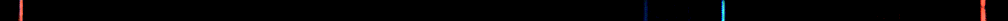
\includegraphics[width=15cm]{H_cut.png}
%   \caption{水素原子のスペクトルの測定結果．一番左端のピークがスリットから入る光のピークである．このピークを基準にしてスペクトル線の波長を測定した．そしてそこから右側に三本のピークが見える．これらのピークがスペクトル線に対応している．なお，この画像はスペクトルを見やすくするために彩度，濃度を調整している．}
%   .\label{fig:H_cut}
%  \end{center}
% \end{figure}
\begin{figure}[H]
 \begin{center}
  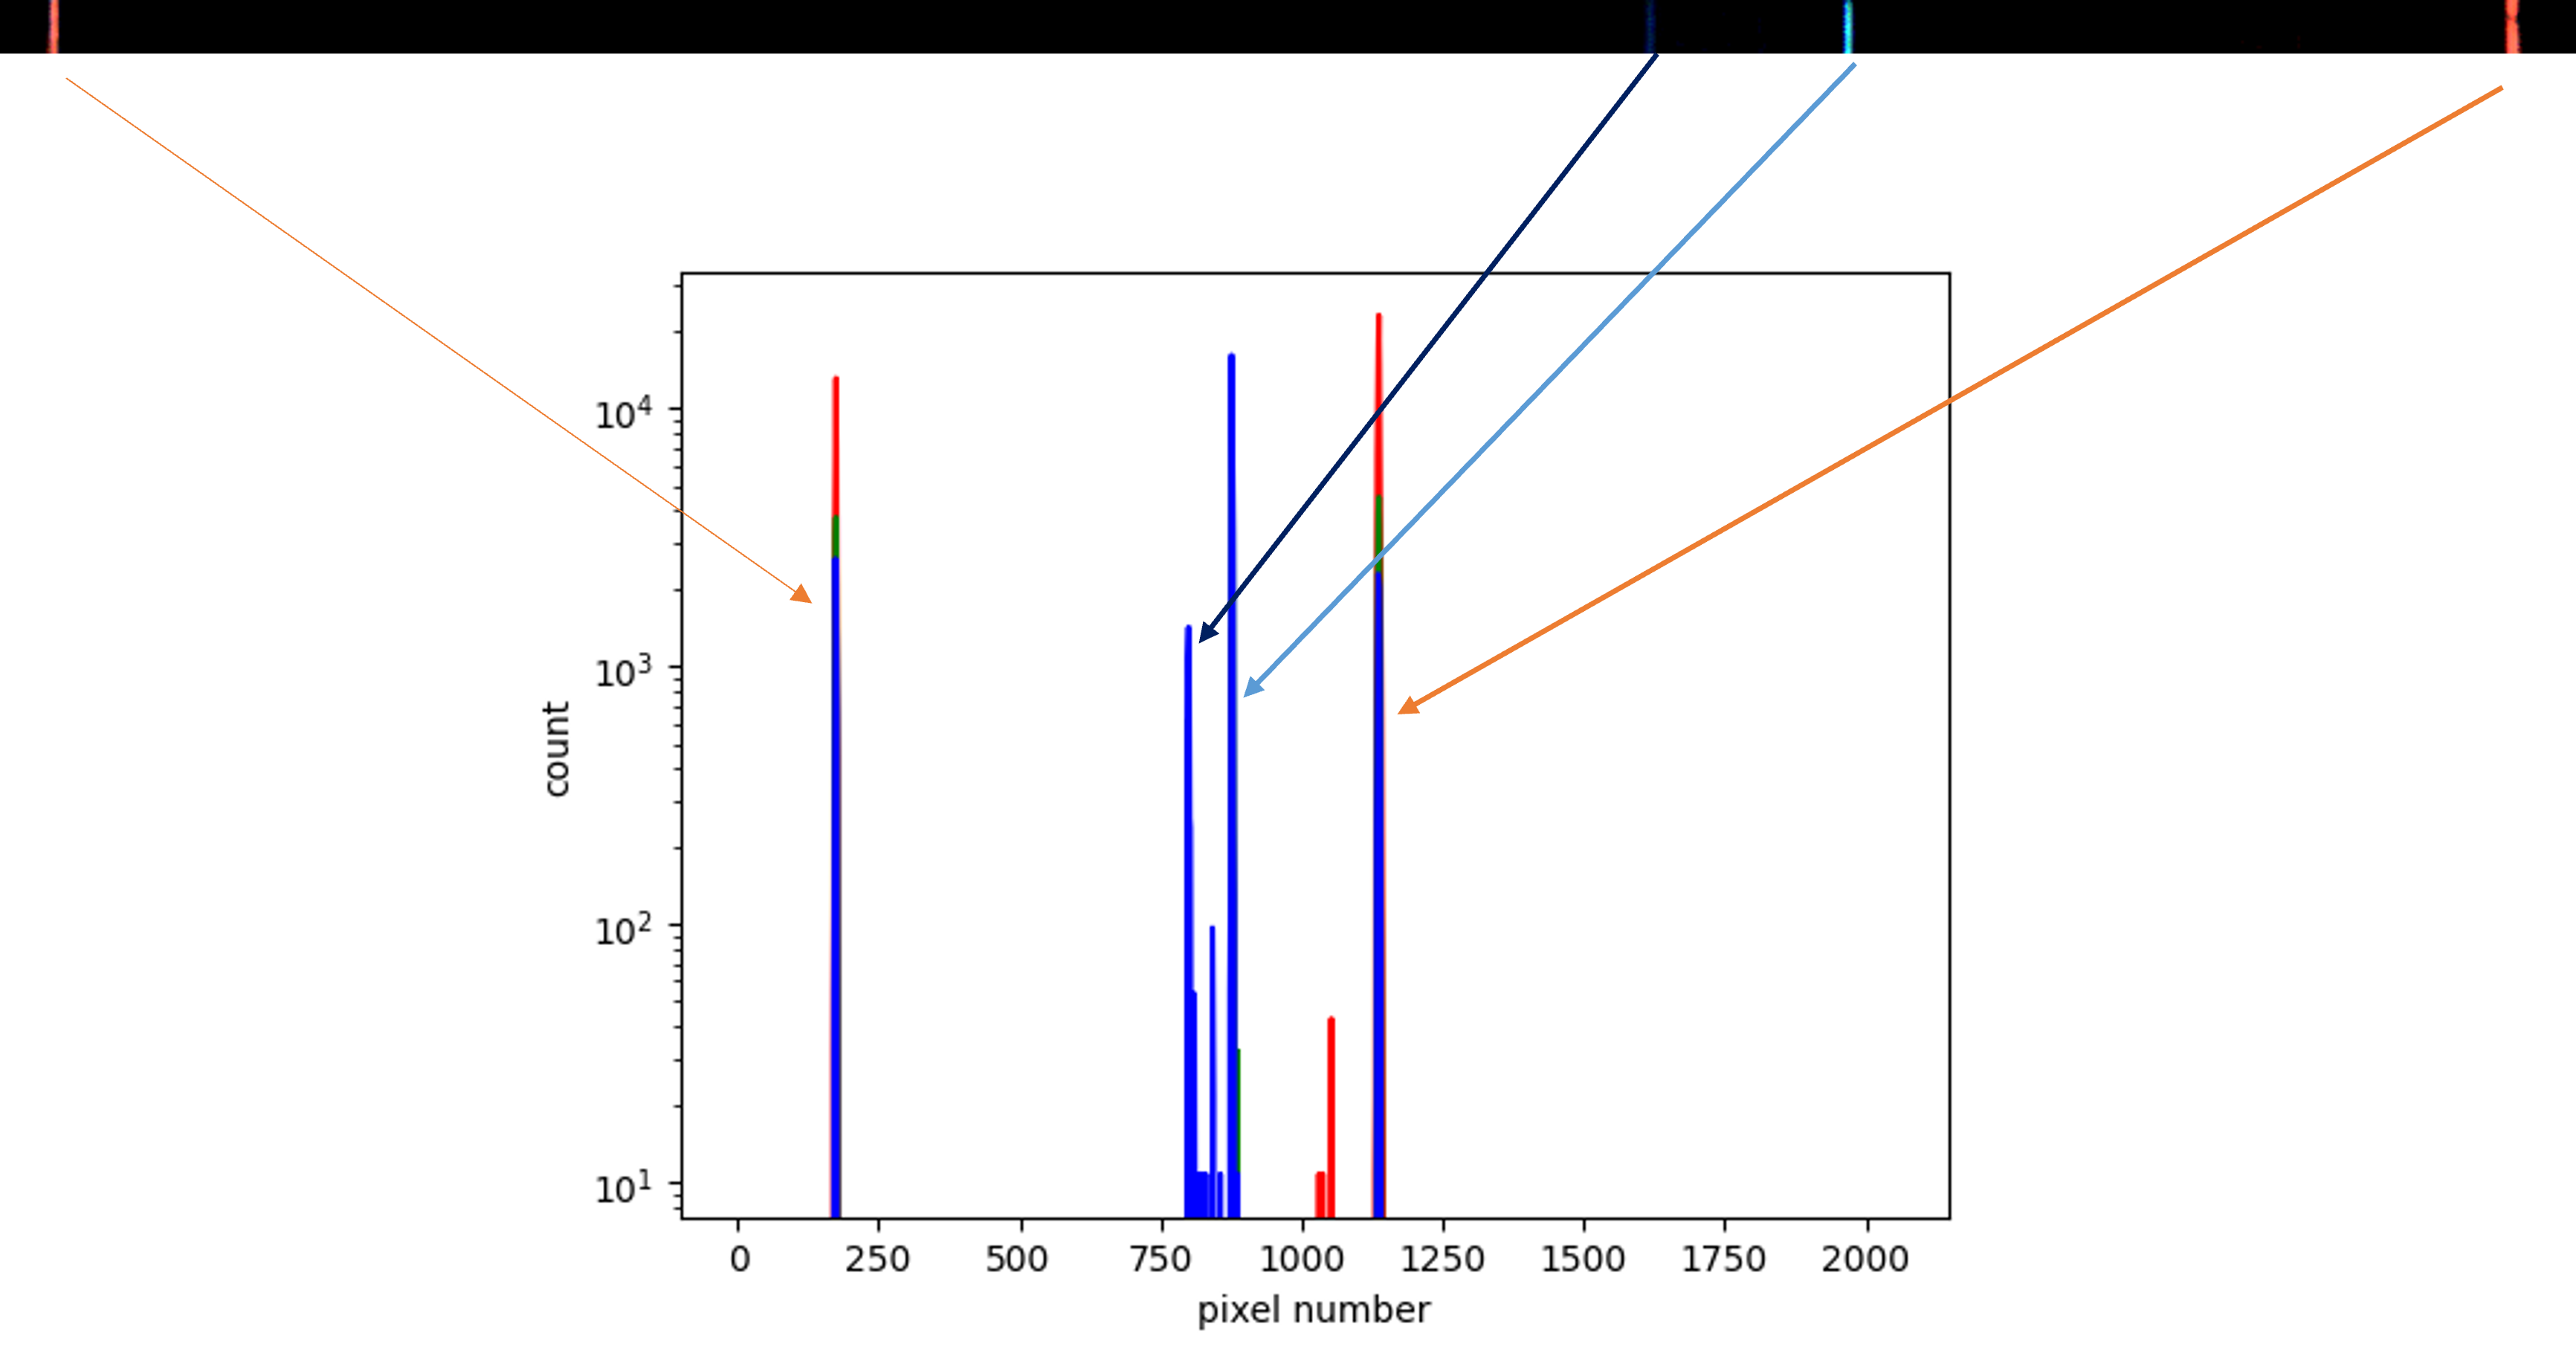
\includegraphics[width=15cm]{H.png}
  \caption{水素原子のスペクトルとそのヒストグラム．縦軸がピークのカウント数を，横軸がピークのピクセルの位置を表している．なお，縦軸は対数スケールである．ピークは各スペクトル線に対応している．Rのヒストグラムは赤色のスペクトル線に対応している．Gのヒストグラムは緑色のスペクトル線に対応している．Bのヒストグラムは青色のスペクトル線に対応している．  また，矢印はスペクトル線とヒストグラムのピークの対応を示している．}
  .\label{fig:H_spectrum}
 \end{center}
\end{figure}
レポートに載せるにあたっては，スペクトルを見やすくするためにカットされた画像は適宜拡大し，彩度，濃度を調整している．一番左のスペクトル線がスリットから入る光のピークである．このピークを基準にしてスペクトル線の波長を測定した．そしてそこから右側に三本のピークが見える．これらのピークがスペクトル線に対応している．図\ref{fig:H_spectrum}は水素原子のスペクトルとそのヒストグラムである．縦軸がピークのカウント数を，横軸がピークのピクセルの位置を表している．なお，縦軸は対数スケールである．ピークは各スペクトル線に対応している．Rのヒストグラムは赤色のスペクトル線に対応している．Gのヒストグラムは緑色のスペクトル線に対応している．Bのヒストグラムは青色のスペクトル線に対応している．

この3本のピークについてR，G，Bのヒストグラムの位置とその平均をまとめた表を以下の表\ref{tab:H_spectrum}に示す．
\begin{table}[htbp]
 \begin{center}
  \begin{tabular}{|c|c|c|c|c|}
    \hline
   スペクトル線 & Rのピーク位置 & Gのピーク位置 & Bのピーク位置& 平均 \\
    \hline
    スリットの位置 & 175 & 175 & 174 & 174.67 \\
   赤色のスペクトル線 & 1137 & 1137 & 1136 & 1136.7 \\
   緑色のスペクトル線 & 877 & 877 & 876 & 876.67 \\
   青色のスペクトル線 & なし & 799 & 800 & 799.50 \\
   \hline
  \end{tabular}
  \caption{水素原子のスペクトル線とそのヒストグラムのピーク位置．単位はPIXELである．カウント数が100以上のもののみを対象としている．なお，青色のスペクトル線についてはRのヒストグラムにはピークが見られなかったため，Rのピーク位置はなしとした．}
  .\label{tab:H_spectrum}
 \end{center}
\end{table}
表\ref{tab:H_spectrum}は水素原子のスペクトル線とそのヒストグラムのピーク位置をまとめたものである．単位はPIXELである．カウント数が100以上のもののみを対象としている．なお，青色のスペクトル線についてはRのヒストグラムにはピークが見られなかったため，Rのピーク位置はなしとした．

次に，ヘリウム原子のスペクトルの測定結果とそのヒストグラムを図\ref{fig:He_spectrum}に示す．
% \begin{figure}[H]
%  \begin{center}
%   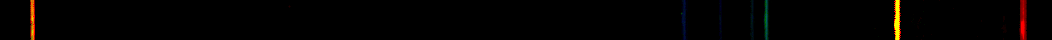
\includegraphics[width=15cm]{He_cut.png}
%   \caption{ヘリウム原子のスペクトルの測定結果．この画像はスペクトルを見やすくするために彩度，濃度を調整している．一番左にスペクトル線がスリットから入る光のピークが見える．このピークを基準にしてスペクトル線の波長を測定した．そしてそこから右側に6本のピークが見える．これらのピークがスペクトル線に対応している．}
%   .\label{fig:He_cut}
%  \end{center}
% \end{figure}
\begin{figure}[H]
  \begin{center}
    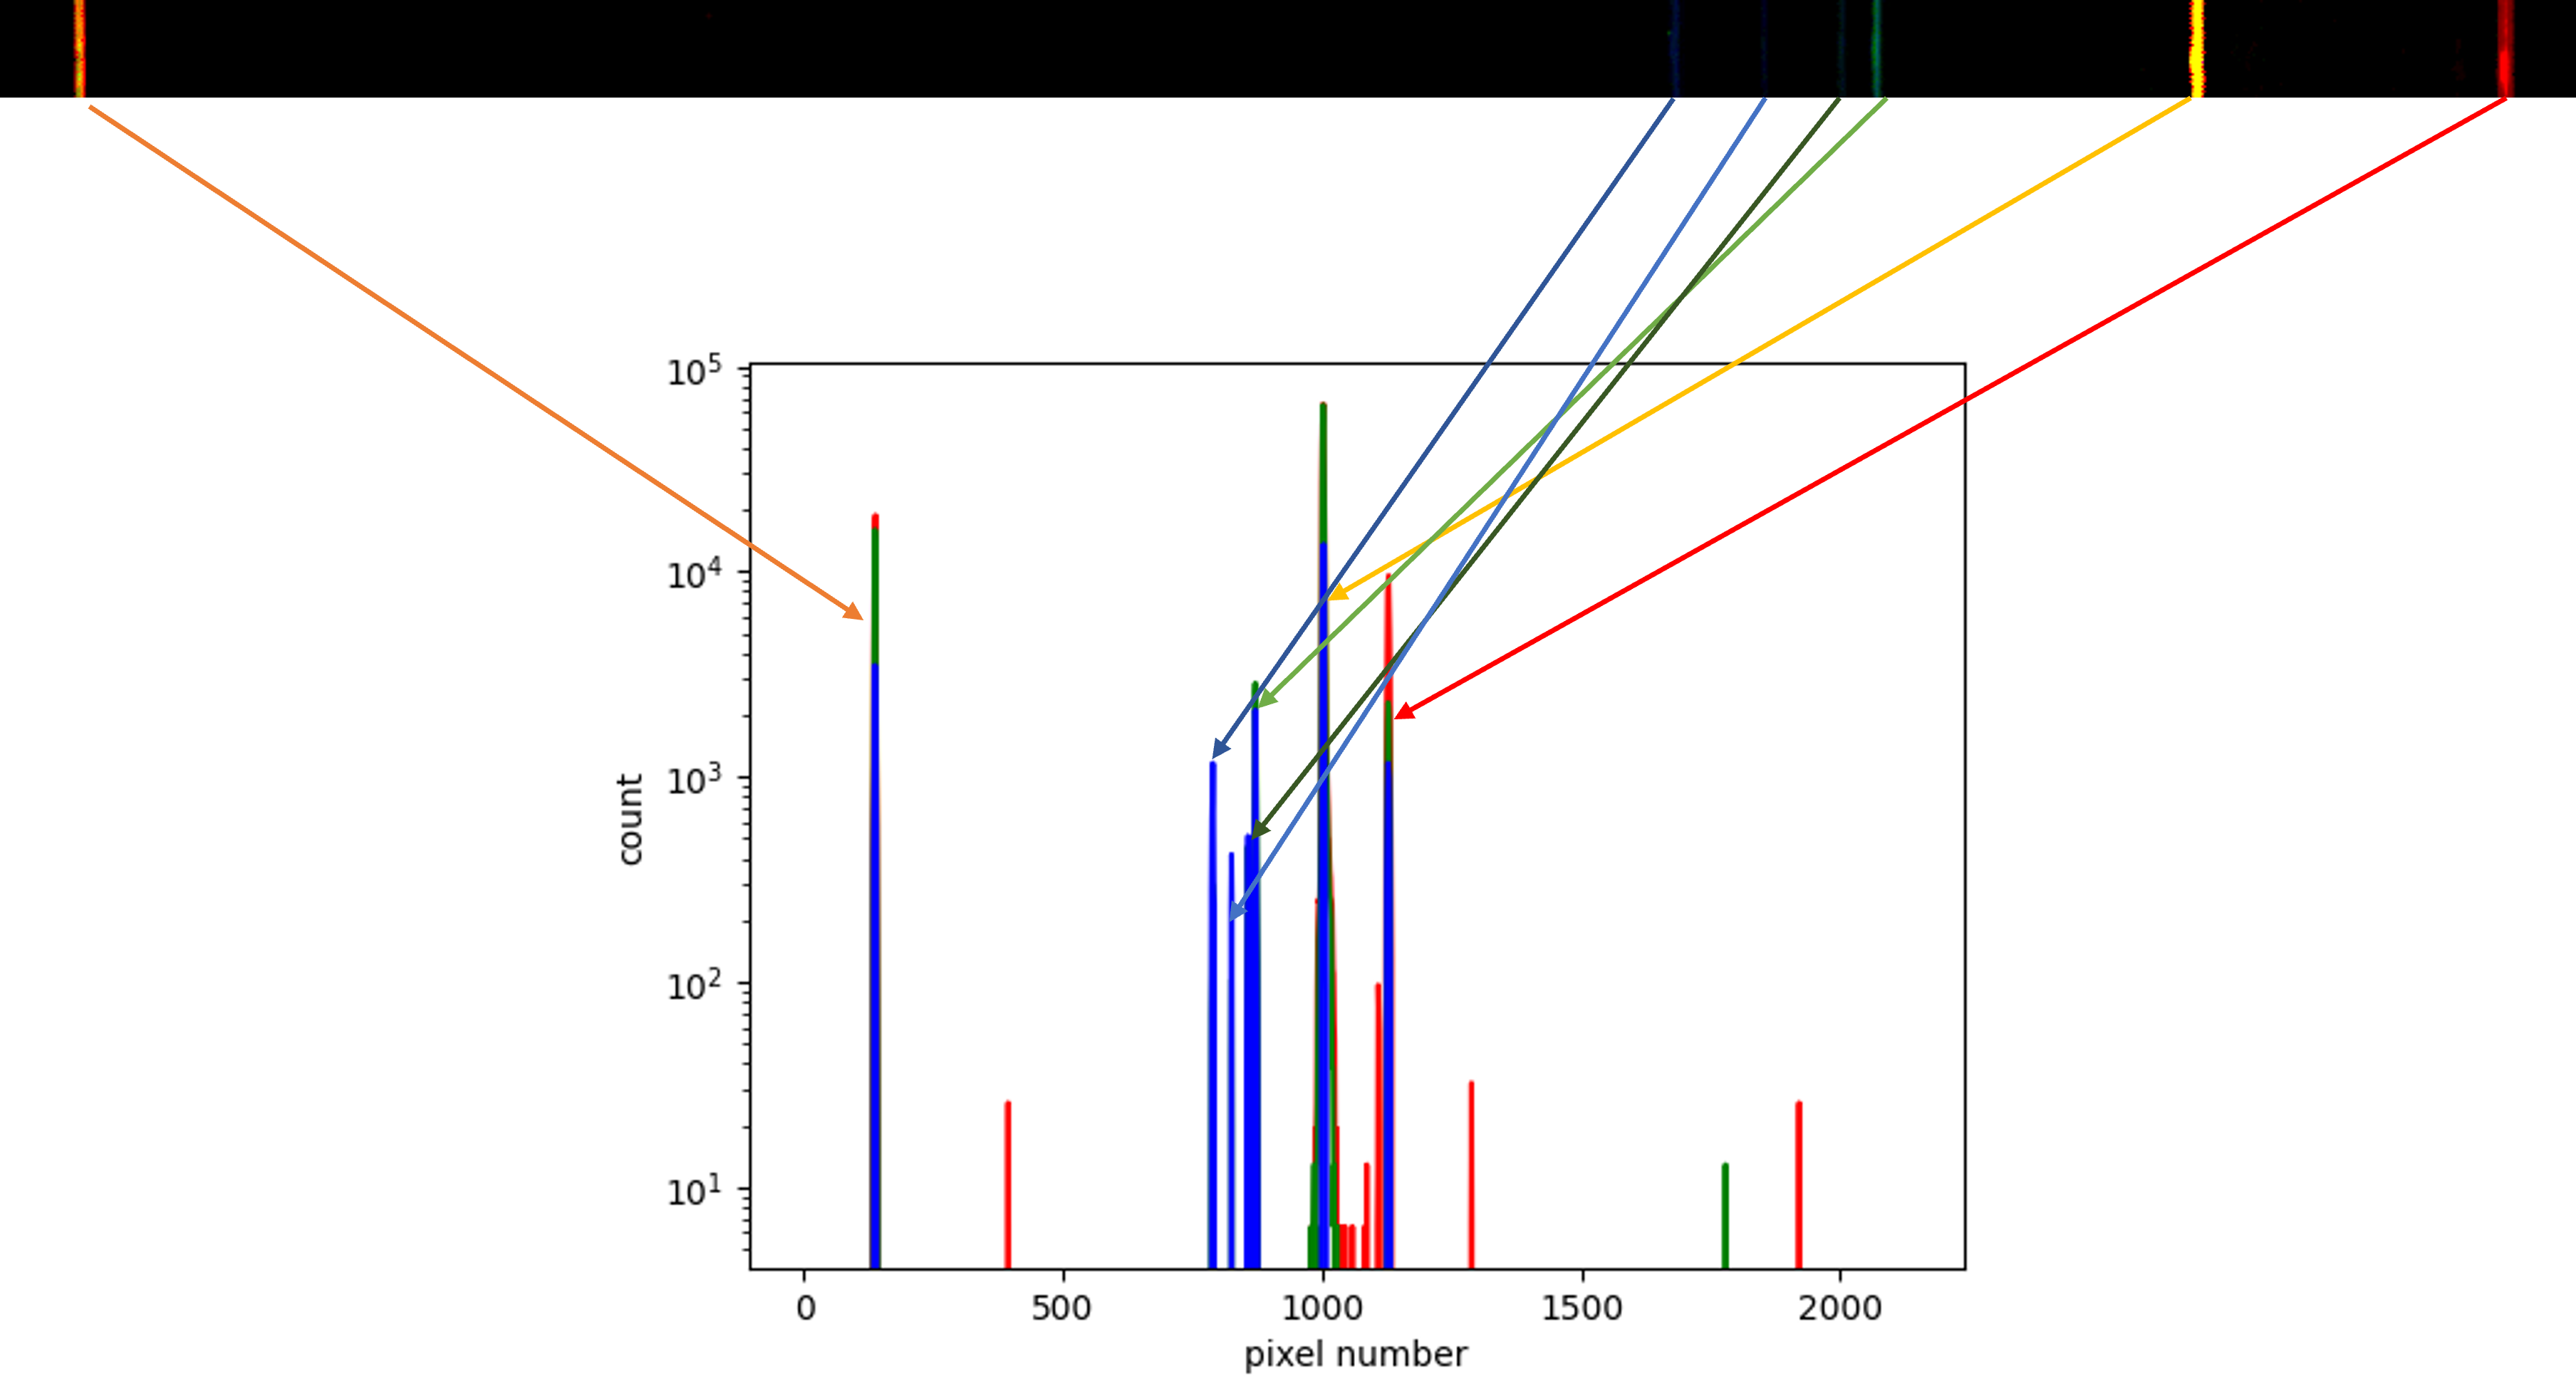
\includegraphics[width=15cm]{He.png}
    \caption{ヘリウム原子のスペクトルとそのヒストグラム．縦軸がピークのカウント数を，横軸がピークのピクセルの位置を表している．なお，縦軸は対数スケールである．ピークは各スペクトル線に対応している．Rのヒストグラムは赤色のスペクトル線に対応している．Gのヒストグラムは緑色のスペクトル線に対応している．Bのヒストグラムは青色のスペクトル線に対応している．矢印はスペクトル線とヒストグラムのピークの対応を示している．}
    .\label{fig:He_spectrum}
  \end{center}
\end{figure}
レポートに載せるにあたっては，スペクトルを見やすくするためにカットされた画像は適宜拡大し，彩度，濃度を調整している．一番左のスペクトル線がスリットから入る光のピークである．このピークを基準にしてスペクトル線の波長を測定した．そしてそこから右側に赤，黄，緑，深緑，青，紫の6本のピークが見える．これらのピークがスペクトル線に対応している．図\ref{fig:He_spectrum}はヘリウム原子のスペクトルとそのヒストグラムである．縦軸がピークのカウント数を，横軸がピークのピクセルの位置を表している．なお，縦軸は対数スケールである．ピークは各スペクトル線に対応している．Rのヒストグラムは赤色のスペクトル線に対応している．Gのヒストグラムは緑色のスペクトル線に対応している．Bのヒストグラムは青色のスペクトル線に対応している．図\ref{fig:He_spectrum}のPIXELが800付近には3つのピークがあることに注意する．

この6本のピークについてR，G，Bのヒストグラムの位置とその平均をまとめた表を以下の表\ref{tab:He_spectrum}に示す．
\begin{table}[htbp]
  \begin{center}
    \begin{tabular}{|c|c|c|c|c|}
       \hline
    スペクトル線 & Rのピーク位置 & Gのピーク位置 & Bのピーク位置& 平均 \\
      \hline
      スリットの位置 & 139 & 138 & 138 & 138.33 \\
    赤色のスペクトル線 & 1129 & 1128& 1128 & 1128.3 \\
    黄色のスペクトル線 & 1003 & 1003 & 1004 & 1003.3\\
    緑色のスペクトル線 & なし & 872 & 872 & 872.00 \\
    深緑色のスペクトル線 & なし & 858 & 858 & 858.00 \\
    青色のスペクトル線 & なし & 826 & 826 & 826.00 \\
    紫色のスペクトル線 & なし & 789 & 790 & 789.50 \\
    \hline
    \end{tabular}
    \caption{ヘリウム原子のスペクトル線とそのヒストグラムのピーク位置．単位はPIXELである．カウント数が100以上のもののみを対象としている．}
    .\label{tab:He_spectrum}
  \end{center}
\end{table}
表\ref{tab:He_spectrum}はヘリウム原子のスペクトル線とそのヒストグラムのピーク位置をまとめたものである．単位はPIXELである．カウント数が100以上のもののみを対象としている．

最後に，LED，白熱電球，水銀灯のスペクトルの観察結果を図\ref{fig:LED}，図\ref{fig:incandescent}，図\ref{fig:mercury}に示す．
\begin{figure}[H]
 \begin{center}
  \includegraphics[width=15cm]{LED_cut.png}
  \caption{LEDのスペクトル．この画像はスペクトルを見やすくするために彩度，濃度を調整している．色が非常に混ざってしまっていてスペクトル線が見えにくい．}
  .\label{fig:LED}
 \end{center}
\end{figure}
\begin{figure}[H]
  \begin{center}
    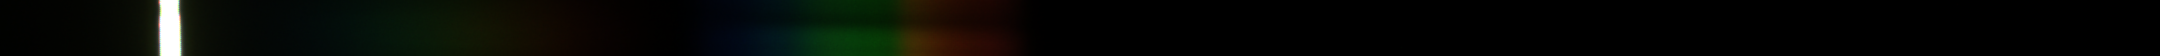
\includegraphics[width=15cm]{Kr_cut.png}
    \caption{白熱電球のスペクトル．この画像はスペクトルを見やすくするために彩度，濃度を調整している．連続的なスペクトルが見える}
    .\label{fig:incandescent}
  \end{center}
\end{figure}
\begin{figure}[H]
  \begin{center}
    
\includegraphics[width=15cm]{Hg_cut.png}
    \caption{水銀灯のスペクトル．この画像はスペクトルを見やすくするために彩度，濃度を調整している．スリット以外に6本のスペクトル線が見える．}
    .\label{fig:mercury}
  \end{center}
\end{figure}
図\ref{fig:LED}はLEDのスペクトルである．この画像はスペクトルを見やすくするために彩度，濃度を調整している．色が非常に混ざってしまっていてスペクトル線が見えにくい．図\ref{fig:incandescent}は白熱電球のスペクトルである．この画像はスペクトルを見やすくするために彩度，濃度を調整している．連続的なスペクトルが見える．図\ref{fig:mercury}は水銀灯のスペクトルである．この画像はスペクトルを見やすくするために彩度，濃度を調整している．スリット以外に赤，橙，黄，薄緑，青紫，紫の6本のスペクトル線が見える．
\section{課題と考察}
この課題及びそれに付帯した考察において，水素原子のスペクトル，ヘリウム原子のスペクトルのPIXELの位置は表\ref{tab:H_spectrum}と表\ref{tab:He_spectrum}に示したもののうち平均を用いることとする．
\subsection{水素原子のスペクトルについて}
\begin{itembox}[l]{演習1}
式\eqref{eq:energy}を用いて主量子数$n$が1から5までのときの水素原子のエネルギー準位$[\text{eV}]$を求めよ．
\end{itembox}
\quad 式\eqref{eq:energy}を用いて主量子数$n$が1から5までのときの水素原子のエネルギー準位は以下のように表される．
\begin{align}
  &E_1 = -1.36 \times 10\, \text{eV},\\
  &E_2 = -3.40  \, \text{eV},\\
  &E_3 = -1.51 \, \text{eV},\\
  &E_4 = -8.50\times10^{-1} \, \text{eV},\\
  &E_5 = -5.44\times10^{-1} \, \text{eV}.
\end{align}
\begin{itembox}[l]{演習2}
バルマー系列に分類されるスペクトルのうち，$n=5\to n=2$，$n=4\to n=2$，$n=3\to n=2$のときのスペクトル線のエネルギーと波長を式\eqref{eq:Rydberg}を用いて求めよ．
\end{itembox}
\quad 式\eqref{eq:Rydberg}と$\hbar c=1.24 \times 10^3 \, \text{eV}\cdot\text{nm}$，$\lambda = \frac{\hbar c}{E}$を用いて，バルマー系列に分類されるスペクトルのうち，$n=5\to n=2$，$n=4\to n=2$，$n=3\to n=2$のときのスペクトル線のエネルギーと波長は以下のように表される．
\begin{align}
  &n=5\to n=2: E = 2.85 \, \text{eV}, \lambda = 4.34\times10^{2} \, \text{nm},\\
  &n=4\to n=2: E = 2.55 \, \text{eV}, \lambda = 4.86\times10^{2} \, \text{nm},\\
  &n=3\to n=2: E = 1.89 \, \text{eV}, \lambda = 6.56\times10^{2} \, \text{nm}.
\end{align}

\begin{itembox}[l]{演習3}
  ピクセルナンバーと波長の関係が線形であると仮定して，水素原子のスペクトルの測定結果がバルマー系列のスペクトル線に対応していることを確認せよ．
\end{itembox}
\quad  赤色のスペクトル線と青色のスペクトル線の差は337.17PIXEL，緑色のスペクトル線と青色のスペクトル線の差は77.167PIXELである．一方，バルマー系列に分類されるスペクトルのうち，$n=5\to n=2$，$n=4\to n=2$，$n=3\to n=2$のときのスペクトル線の波長はそれぞれ434nm，486nm，656nmである．このため，赤色のスペクトル線と青色のスペクトル線の差は222nm，緑色のスペクトル線と青色のスペクトル線の差は52.0nmである．ところで，これらの値の比をとってみると，
\begin{align}
  &\frac{337.17}{77.167} \simeq 4.37,\\
  &\frac{222}{52.0} \simeq 4.27.
\end{align}
となり，PIXELの差の比と波長の差の比は近い値をとることがわかる．このことから，数学的にもピクセルナンバーと波長の関係が線形であると仮定してさしつかえないことがわかる．

\begin{itembox}[l]{演習4}
\quad 水素原子のスペクトルとバルマー系列のスペクトル線の波長を用いて，ピクセルナンバーと波長の関係をグラフにプロットし，線形回帰を行うことでピクセルナンバーと波長の関係を求めよ．なお，$y=a(x-x_0)+b$の形で表される線形関係を仮定し，$x_0$はスリットから入る光のピークの位置とすること．
\end{itembox}
 表\ref{tab:H_spectrum}の水素原子のスペクトル線とそのヒストグラムのピーク位置を用いて，ピクセルナンバーと波長の関係をグラフにプロットしたものを図\ref{fig:pixel_wavelength}に示す．縦軸は波長(nm)を，横軸はピクセルナンバーからスリットから入る光のピークの位置を引いたものである．
\begin{figure}[htbp]
  \begin{center}
    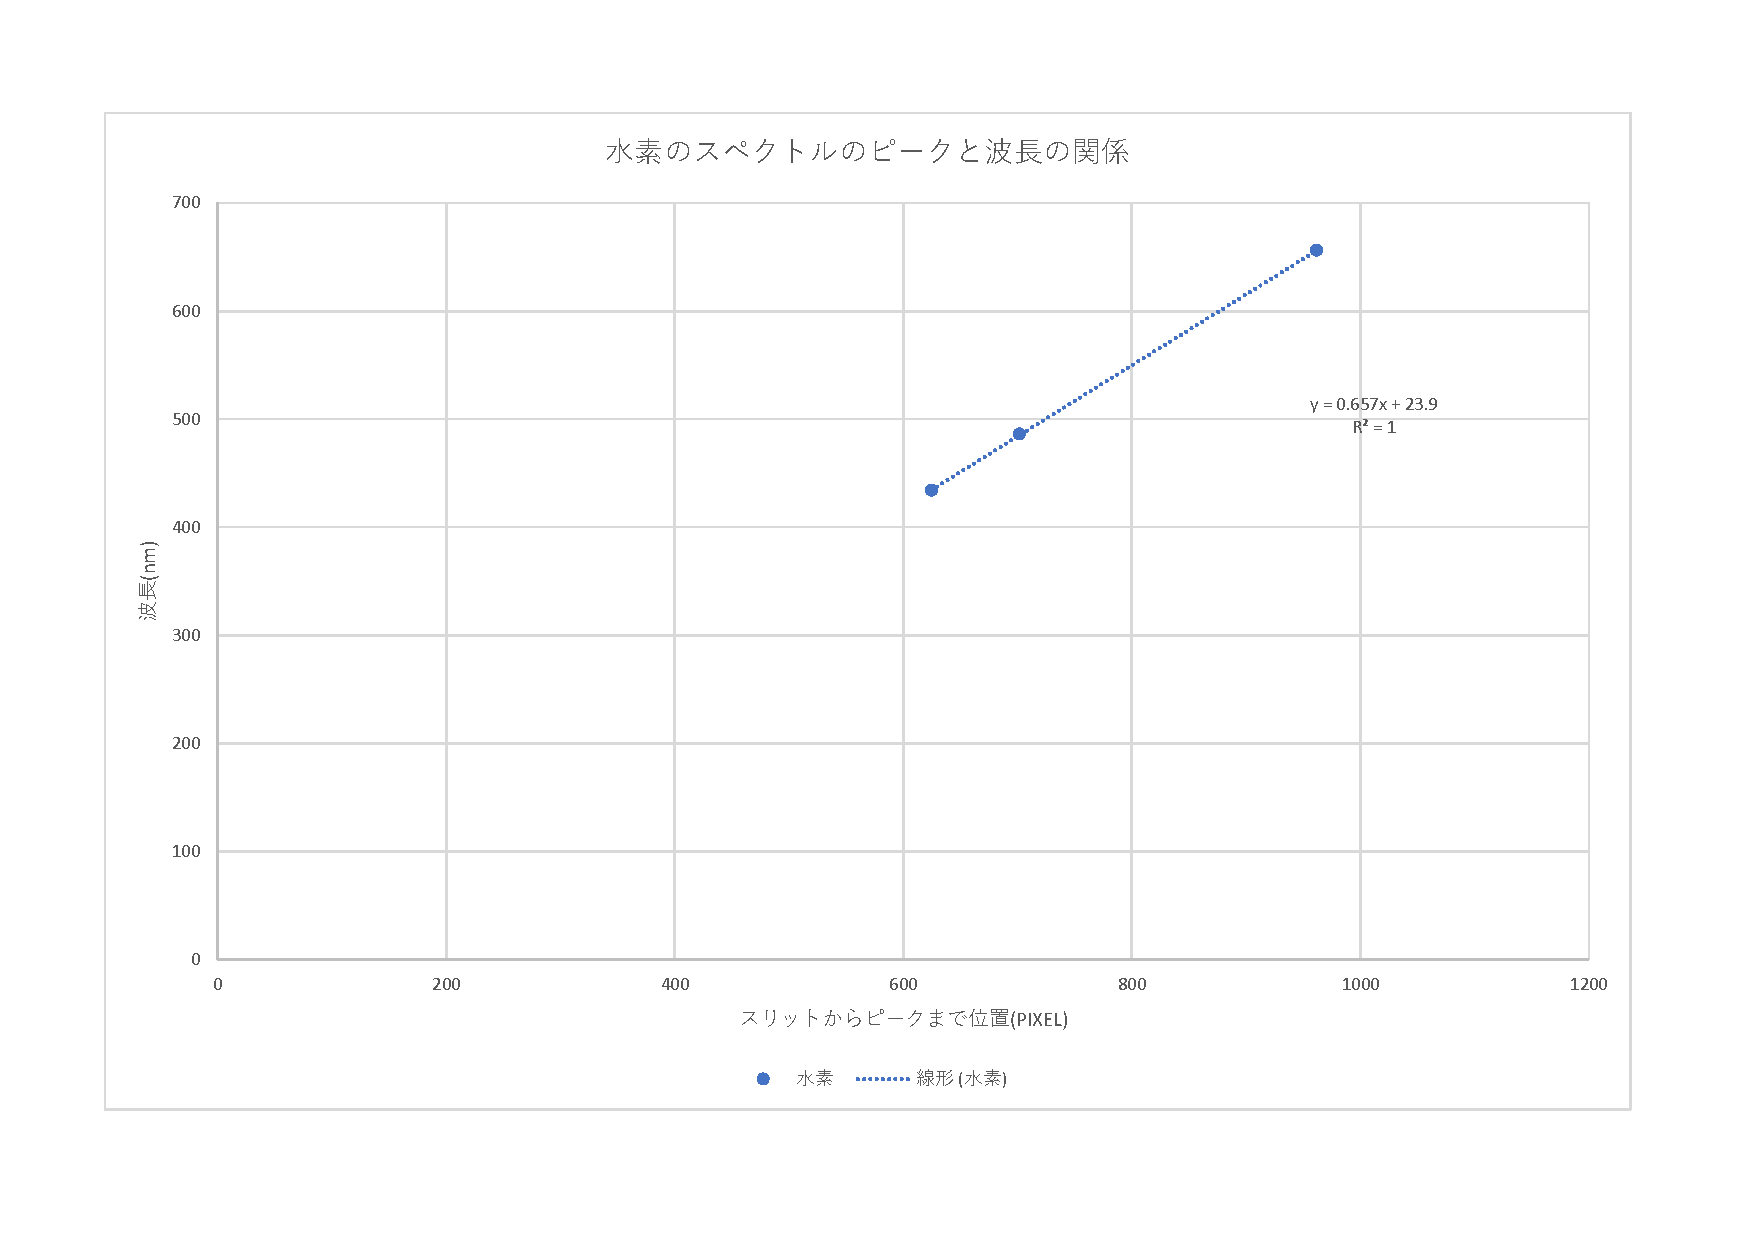
\includegraphics[width=15cm]{H_line.pdf}
    \caption{ピクセルナンバーと波長の関係をグラフにプロットしたもの．縦軸は波長(nm)を，横軸はピクセルナンバーからスリットから入る光のピークの位置を引いたものである．このグラフに線形回帰を行うことで，ピクセルナンバーと波長の関係を求めることができる．その結果は$y=0.657(x-174.67)+23.9$である．}
    .\label{fig:pixel_wavelength}
  \end{center}
\end{figure}
このグラフに線形回帰を行うことで，ピクセルナンバーと波長の関係は以下のように表される．
\begin{equation}
  y=0.657(x-x_0)+23.9\,.\label{eq:pixel_wavelength}
\end{equation}
ここで，$x_0$はスリットから入る光のピークの位置である．この式\eqref{eq:pixel_wavelength}を用いて，ヘリウム原子のスペクトル線の波長を測定することができる．
\subsection{ヘリウム原子のスペクトルについて}
\begin{itembox}[l]{演習1}
  ヘリウム原子のスペクトル線の波長を式\eqref{eq:pixel_wavelength}を用いて算出せよ．
\end{itembox}
\quad 水素原子のスペクトルではスリットの位置は174.67PIXELであった．一方，ヘリウム原子のスペクトルではスリットの位置は138.33PIXELであった．分光器とカメラに触れずにスペクトル管を交換したことを踏まえると，このスリットの位置のずれは画像編集ソフトで画像をカットしたときに生じたものであると考えられる．この際画像の拡大縮小を行っていない．したがってスリット柄木田光と回折像の位置関係にずれはない．以上を踏まえるとヘリウムの分析においては式\eqref{eq:pixel_wavelength}の$x_0$は138.33となる．

表\ref{tab:He_spectrum}のヘリウム原子のスペクトル線とそのヒストグラムのピーク位置を用いて，式\eqref{eq:pixel_wavelength}を算出した結果を以下の表\ref{tab:He_wavelength}に示す．
\begin{table}[htbp]
  \begin{center}
    \begin{tabular}{|c|c|c|c|}
       \hline
    スペクトル線 & PIXEL &波長(nm) & エネルギー(eV) \\
      \hline
    赤色のスペクトル線 & 990 & 675 & 1.84\\
    黄色のスペクトル線 & 865 & 592 & 2.09 \\
    緑色のスペクトル線 & 734 & 506 & 2.45 \\
    深緑色のスペクトル線 & 720 & 497 & 2.50 \\
    青色のスペクトル線 & 688 & 476 & 2.61 \\
    紫色のスペクトル線 & 651 & 452 & 2.74 \\
    \hline
    \end{tabular}
    \caption{ヘリウム原子のスペクトル線とその波長．単位はnmである．}
    .\label{tab:He_wavelength}
  \end{center}
\end{table}

\begin{itembox}[l]{演習2-(a)}
  電子間相互作用を考慮しない近似的なエネルギー準位は式\eqref{eq:He_approximate_energy2}で表される．
  \begin{equation}
    E_n = -AZ^2\left(\frac{1}{n_1^2} + \frac{1}{n_2^2}\right)\,.\label{eq:He_approximate_energy2}
  \end{equation}
  ここで，$A$は定数である．摂動法や変分法で得られた基底状態のエネルギーから$A$を求めよ．
\end{itembox}
\quad $Z=2$，$n_1=n_2=1$とし，変分法のエネルギー$-77.5$eVと摂動法のエネルギー$-78.83$eVを用いて式\eqref{eq:He_approximate_energy2}から$A$を求めると，変分法のエネルギーからは$A=9.69$eV，摂動法のエネルギーからは$A=9.35$eVとなる．
\begin{itembox}[l]{演習2-(b)}
  全問の結果を利用し，励起状態($n=2\sim 5$)のエネルギー準位を式\eqref{eq:He_approximate_energy2}を用いて求めよ．
\end{itembox}
\quad $A=9.69$eVと$A=9.35$eVを用いて式\eqref{eq:He_approximate_energy2}から励起状態($n=2\sim 5$)のエネルギー準位を求めると，表\ref{tab:He_energy}のようになる．
\begin{table}[htbp]
  \begin{center}
    \begin{tabular}{|c|c|c|}
       \hline
    主量子数$n$ & 摂動法:$A=9.35$eVのときのエネルギー準位(eV) & 変分法:$A=9.69$eVのときのエネルギー準位(eV) \\
      \hline
    2 & -46.8 & -48.4\\
    3 & -41.6 & -43.1\\
    4 & -39.8 & -41.2\\
    5 & -38.9 & -40.3\\
    \hline
    \end{tabular}
    \caption{励起状態($n=2\sim 5$)のエネルギー準位．単位はeVである．}
    .\label{tab:He_energy}
  \end{center}
\end{table}

\begin{itembox}[l]{演習2-(c)}
  ヘリウム原子のスペクトル線の波長と励起状態のエネルギー準位を用いて，ヘリウム原子のスペクトル線の波長を求めよ．ただし，バルマー系列に分類されるスペクトル線のうち，$n=5\to n=2$，$n=4\to n=2$，$n=3\to n=2$のときのスペクトル線のエネルギーと波長を式\eqref{eq:Rydberg}を用いて求めたときの値を用いること．
\end{itembox}
\quad ヘリウム原子のスペクトル線の波長と励起状態のエネルギー準位を用いて，ヘリウム原子のスペクトル線のエネルギーと波長を求めると，表\ref{tab:He_spectrum_energy}表\ref{tab:He_spectrum_wavelength}のようになる．
\begin{table}[htbp]
  \begin{center}
    \begin{tabular}{|c|c|c|}
       \hline
    スペクトル線 & 摂動法:$A=9.35$eVのときのエネルギー(eV) & 変分法:$A=9.69$eVのときのエネルギー(eV) \\
      \hline
    $n=5\to n=2$ & 7.86 & 8.14\\
    $n=4\to n=2$ & 7.02 & 7.27\\
    $n=3\to n=2$ & 5.20 & 5.38\\
    \hline
    \end{tabular}
    \caption{ヘリウム原子のスペクトル線のエネルギー．単位はeVである．}
    .\label{tab:He_spectrum_energy}
  \end{center}
\end{table}
\begin{table}[htbp]
  \begin{center}
    \begin{tabular}{|c|c|c|}
       \hline
    スペクトル線 & 摂動法:$A=9.35$eVのときの波長(nm) & 変分法:$A=9.69$eVのときの波長(nm) \\
      \hline
    $n=5\to n=2$ & 158 & 152\\
    $n=4\to n=2$ & 177 & 171\\
    $n=3\to n=2$ & 239 & 230\\
    \hline
    \end{tabular}
    \caption{ヘリウム原子のスペクトル線の波長．単位はnmである．}
    .\label{tab:He_spectrum_wavelength}
  \end{center}
\end{table}
\begin{itembox}[l]{演習2-(d)}
  ヘリウム原子のスペクトル線の波長を実験で測定した値と比較せよ．
\end{itembox}
 まず，表\ref{tab:He_spectrum_wavelength}の値は，可視光の波長が約400nmから約700nmの範囲にあることを踏まえると，非常に小さすぎることがわかる．言い換えればエネルギーが大きすぎるということになる．一方で表\ref{tab:He_wavelength}の値は、可視光の波長が約400nmから約700nmの範囲にあることを踏まえると、妥当な値であることがわかる．このことから、ヘリウム原子のスペクトル線の波長を実験で測定した値と比較すると、近似的な計算結果は実験で測定した値と大きく乖離していることがわかる．この乖離について，エネルギーの面から考えてみる．表\ref{tab:He_wavelength}のエネルギーの値が$1.84$eVから$2.74$eVの範囲にある．一方で表\ref{tab:He_spectrum_energy}のエネルギーの値が$5.20$eVから$8.14$eVの範囲にあり，準位の幅が表\ref{tab:He_wavelength}と比較して約3倍から約4倍の範囲にあることがわかる．このことから、近似的な式\eqref{eq:He_approximate_energy2}では予測できないエネルギー準位の分裂が存在していることがわかる．
 
 このエネルギー準位の分裂は、電子間相互作用とスピン軌道相互作用の両方が寄与していると考えられる．特に，電子のスピンが平行(1重項)であるときと反平行(3重項)であるときでは同じ主量子数であってもエネルギー準位が分裂することが知られている．このようなエネルギー準位の分裂は、近似的な式\eqref{eq:He_approximate_energy2}では考慮されていないため、近似的な計算結果と実験で測定した値が大きく乖離していると考えられる．
\begin{itembox}[l]{演習3}
  実験テキスト表5.1と比較して測定で得られたスペクトル線の波長がどのような遷移に対応しているかを考察せよ．
\end{itembox}
\quad 実験テキスト表5.1の波長をエネルギーに変換したものと表\ref{tab:He_wavelength}の値を比較し，表\ref{tab:He_transition}に示す．
\begin{table}[htbp]
  \begin{center}
    \begin{tabular}{|c|c|c|c|c|}
       \hline
    番号 & 波長(nm) & エネルギー(eV) & 遷移 & 対応する可能性のある波長 \\
      \hline
    A & 402 & 3.08 & $5d\to 2p$三重項& なし\\
    B & 412 & 3.01 & $5s\to 2p$三重項& なし\\
    C & 438 & 2.83 & $5d\to 2p$一重項& なし\\
    D & 443 & 2.80 & $5s\to 2p$一重項& なし\\
    E & 447 & 2.77 & $4d\to 2p$三重項& 452\\
    F & 471 & 2.63 & $4s\to 2p$三重項& 476\\
    G & 492 & 2.52 & $4d\to 2p$一重項& 497\\
    H & 501 & 2.48 & $3p\to 2p$一重項& 506,497\\
    I & 504 & 2.46 & $4s\to 2p$一重項& 506,497\\
    J & 587 & 2.11 & $3d\to 2p$三重項& 592\\
    K & 667 & 1.86 & $3d\to 2p$一重項& 675\\
    \hline
    \end{tabular}
    \caption{実験テキスト表5.1の波長をエネルギーに変換したものと表\ref{tab:He_wavelength}の値を比較したもの．この表の遷移は実験テキスト表5.1の遷移である．対応する可能性のある波長は表\ref{tab:He_wavelength}の値である．}
    .\label{tab:He_transition}
  \end{center}
\end{table}
エネルギーの値の差が$0.05$eV未満のものを対応する可能性のある波長とした．J，Kの遷移は$675$nm，$592$nmの波長に対応するとしたが，これらの遷移確率が高いことと図\ref{fig:He_spectrum}において赤色と黄色が比較的輝度が高いこととつじつまが合う．前問で述べた通り，スピンの状態によるエネルギー準位の分裂が存在していることがわかる．特に，Jの遷移は$3d\to 2p$三重項であるのに対してKの遷移は$3d\to 2p$一重項であり，三重項の遷移の方がエネルギーが大きくなっているのはスピンが平行であるときの方がエネルギーが大きくなることとつじつまが合う．


\subsection{LED，白熱電球，水銀灯のスペクトルについて}
私が持っているパソコンがLINUXOSではないため，LED，白熱電球，水銀灯の波長の測定を行うことはできなかった．よってここでは定性的な考察を行う．まず，lEDについて，図\ref{fig:LED}のスペクトルを見ると，青色$\sim$黄色のスペクトルにかけて色が非常に混ざっている．これは近年よく見られる青色と黄色のLEDを組み合わせた白色LEDであることが原因であると考えられる．次に，白熱電球について，図\ref{fig:incandescent}のスペクトルを見ると，連続的なスペクトルが見える．これは白熱電球が黒体放射に近いスペクトルを持つためであると考えられる．最後に，水銀灯について，図\ref{fig:mercury}のスペクトルを見ると，赤，橙，黄，薄緑，青紫，紫の6本のスペクトル線が見える．このスペクトルの特徴は図\ref{fig:mercury_spectrum}に示されている水銀灯のスペクトルの特徴と一致している．このことから，水銀灯のスペクトルは水銀原子のスペクトル線に対応していると考えられる．
\begin{figure}[H]
  \begin{center}
    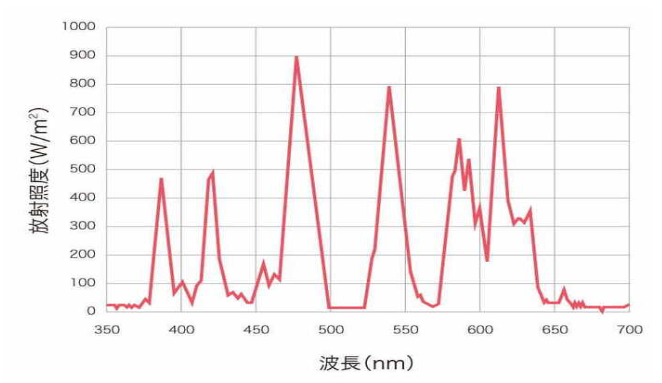
\includegraphics[width=10cm]{Hg_spectrum.png}
    \caption{水銀灯のスペクトルの特徴．縦軸が放射照度，横軸が波長．このスペクトルの特徴は図\ref{fig:mercury}に示されている水銀灯のスペクトルの特徴と一致している．このことから，水銀灯のスペクトルは水銀原子のスペクトル線に対応していると考えられる．\cite{KLV_Hg}より引用．}
    .\label{fig:mercury_spectrum}
  \end{center}  
\end{figure}
\section{結論・まとめ}
本実験では，水素原子のスペクトルとヘリウム原子のスペクトルを測定し，それらのスペクトル線の波長を求めた．また，LED，白熱電球，水銀灯のスペクトルを観察した．水素原子のスペクトルでは，バルマー系列に分類されるスペクトル線が観察され，ピクセルナンバーと波長の関係が線形であることが確認された．ヘリウム原子のスペクトルでは，近特に励起状態より上の準位では近似法を用いて計算した準位の値が実験値と一致しないことがわかった．これがスピン軌道相互作用によるエネルギー準位の分裂が存在していることと一致する．LEDのスペクトルは製品の作られ方に依存し，白熱電球のスペクトルでは黒体放射のような連続的なスペクトルが見えることがわかった．水銀灯のスペクトルでは赤，橙，黄，薄緑，青紫，紫の6本のスペクトル線が見えることがわかり，水銀灯のスペクトルは水銀原子のスペクトル線に対応していると考えられることがわかった．



%参考文献
\begin{thebibliography}{20}
\bibitem{text}
東京科学大学理学院編，大学院物理基本実験，2026
\bibitem{igi_kawai}
猪木 慶治,，川合 光，量子力学I\hspace{-1.2pt}I，講談社，1994，東京

\bibitem{kondou}
近藤 慶一，量子力学講義I\hspace{-1.2pt}I，共立出版，2023，東京

\bibitem{TOSHIBA}
\url{https://www.tlt.co.jp/tlt/lighting_design/proposal/led_basics/led_w_emission.htm}
アクセス日:2026-05-07

\bibitem{KLV_Hg}
\url{https://www.klv.co.jp/corner/what-is-mercury-lamp.html}
アクセス日:2026-05-07

\bibitem{KLV_incandescent}
\url{https://www.klv.co.jp/corner/light-source-wavelength-characteristics.html}
アクセス日:2026-05-07



\end{thebibliography}

\end{document}